%%%%%%%%%%%%%%%%%%%%%%% file template.tex %%%%%%%%%%%%%%%%%%%%%%%%%
%
% This is a general template file for the LaTeX package SVJour3
% for Springer journals.          Springer Heidelberg 2010/09/16
%
% Copy it to a new file with a new name and use it as the basis
% for your article. Delete % signs as needed.
%
% This template includes a few options for different layouts and
% content for various journals. Please consult a previous issue of
% your journal as needed.
%
%%%%%%%%%%%%%%%%%%%%%%%%%%%%%%%%%%%%%%%%%%%%%%%%%%%%%%%%%%%%%%%%%%%
%
% First comes an example EPS file -- just ignore it and
% proceed on the \documentclass line
% your LaTeX will extract the file if required

%\begin{figure}
%  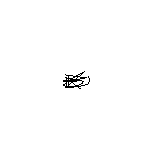
\includegraphics[width=2cm\textwidth, height=2cm \textheight]{file_pdf/signature.pdf}}
%\end{figure} 



\begin{filecontents*}{example.eps}
%!PS-Adobe-3.0 EPSF-3.0
%%BoundingBox: 19 19 221 221
%%CreationDate: Mon Sep 29 1997
%%Creator: programmed by hand (JK)
%%EndComments
gsave
newpath
  20 20 moveto
  20 220 lineto
  220 220 lineto
  220 20 lineto
closepath
2 setlinewidth
gsave
  .4 setgray fill
grestore
stroke
grestore
\end{filecontents*}
%
\RequirePackage{fix-cm}
%
%\documentclass{svjour3}                     % onecolumn (standard format)
%\documentclass[smallcondensed]{svjour3}     % onecolumn (ditto)
\documentclass[smallextended]{svjour3}       % onecolumn (second format)

%\documentclass[twocolumn]{svjour3}          % twocolumn
%
\smartqed  % flush right qed marks, e.g. at end of proof
%
\usepackage[francais]{babel}
\usepackage{graphicx}
\usepackage[utf8]{inputenc}  
\usepackage{eurosym}
\usepackage{rotfloat}
\usepackage{amsmath}
\usepackage{amssymb}
%
% \usepackage{mathptmx}      % use Times fonts if available on your TeX system
%
% insert here the call for the packages your document requires
%\usepackage{latexsym}
% etc.
%
% please place your own definitions here and don't use \def but
% \newcommand{}{}
%
% Insert the name of "your journal" with
% \journalname{myjournal}
%
\setlength\abovecaptionskip{0.25ex}
\setlength\belowcaptionskip{0.25ex}
\begin{document}

\title{Vers la traduction automatique de programme C en clauses de Horn\smallberak%\thanks{Grants or other notes

%about the article that should go on the front page should be
%placed here. General acknowledgments should be placed at the end of the article.}
}

%\subtitle{Do you have a subtitle?\\ If so, write it here}

%\titlerunning{Short form of title}        % if too long for running head

\author{RAYNAUD Paul  \\ \and \\
        Dirigé par : P\'{E}RIN Michaël  %if many names separate them with \and.
}

%\authorrunning{Short form of author list} % if too long for running head

\institute{Paul RAYNAUD \at
              361 allée de Hector Berlioz 38400 \\
              Tel.: 06 15 54 38 90\\
              \email{paul.raynaud66@hotmail.fr}           %  \\
%             \emph{Present address:} of F. Author  %  if needed
}

\date{Juin 2018}
% The correct dates will be entered by the editor

\maketitle{\bf Compilateur C vers clauses de Horn\smallbreak}

\begin{abstract}
%	Être capable de vérifier si un programme réalise ce que nous souhaitons de manière automatique est quelque chose d'utile, car au lieu de montrer nos erreurs ou l'absence d'erreurs que nous capturons avec des tests, nous sommes capables de montrer la correction du programme. Fort de cette preuve nous pouvons assurer que notre programme réalise effectivement la spécification décrit.


	Vérifier de manière automatique si un programme réalise sa spécification nous permet de montrer quelque chose de plus fort que l'absence de certaines erreurs, nous sommes capables de montrer la correction du programme. 
	Nous chercherons donc à prouver à partir d'un programme source si celui ci est capable de satisfaire les propriétés qui lui sont attachées ou non le tout de manière automatique.
	%Nous nous baserons sur des principes déjà connu tel que la Logic de Hoare, et l'étude de graphe de flot de contrôle pour générer sous forme de clauses de Horn les formules logiques associés à un programme.
		Nous nous baserons sur des principes déjà connus tel que la Logic de Hoare, et l'étude de graphe de flot de contrôle pour générer des clauses de Horn.
	Une fois ces formules logiques générées nous aurons recours à un SMT solver pour résoudre les-dites formules.
	Mon stage étant sur plus d'un mois (magistère) les résultats actuels se limitent à la mise en place de bonnes conditions pour travailler réellement sur le sujet.


%\underline{Dois-je laisser les définitions dans ce paragraphe ou dans un autre}

%Insert your abstract here. Include keywords, PACS and mathematical subject classification numbers as needed.
\keywords{CompCert \and Program verification \and Automatic Verification }
% \PACS{PACS code1 \and PACS code2 \and more}
% \subclass{MSC code1 \and MSC code2 \and more}
\end{abstract}

\section{L'intêret de vérifier un programme}
\label{sec:1}
\subsection{Les risques liés à l'informatique}
	Les bugs sur des systèmes informatiques sont quelques choses de banalisés, mais l'informatique étant présente partout, et notamment dans des domaines critiques (santé, embarqué, ...), il est indispensable de prouver qu'un logiciel est capable de répondre aux contraintes décrites dans sa spécification.

\label{sec:2}
\subsection{Explication brève des choix du projet}
	
	L'objectif à long terme est de réaliser un outil capable de vérifier à la compilation si un programme satisfait des propriétés de sûreté telles que l'absence de division par zéro, l'absence de débordement de tableaux, ...
	Le language C est le plus utilisé dans les systèmes embarqués critiques, par conséquent nous travaillerons sur un vérificateur de programme C.

	Les principes de vérification ont été décris pour la première fois en 1969 dans "An Axiomatic Basis for Computer Programming", par Charles A.R. Hoare inspiré des travaux de Floyd.
	La Logique de Hoare est un outil de vérification formelle d'un programme basé sur la sémantique du language dans lequel est écrit le programme. 
	Il est naturellement plus simple d'utiliser ces principes sur des graphes de flot de contrôle pour générer les clauses de Horn. 
	Un CFG est une représentation d'un programme permettant de visualiser les chemins qu'il peut atteindre.
	Les clauses de Horn sont des implications logiques quantifiées universellement dont les prémisses et la conclusion sont des prédicats de base.
	Ces clauses sont par ailleurs l'une des entrées standards utilisées par de nombreux SMT solvers. 
	Un SMT-solver est un SAT-Solver, un logiciel prenant en entrée une formule logique comme les clauses de Horn et qui en sortie répond si cette formules est satisfaisable ou non. (ex Alt-Ergo)


%	- Le language C étant un (vieux/bas niveau) language 
	La norme C est floue sur certains points et laisse place à l'interprétation, de ce fait la sémantique varie subtillement d'un compilateur C à un autre.
D'autres parts il existe des erreurs de compilation appelées: miscompilations. Celles-ci générent des éxécutions incorrectes de programmes pourtant corrects. C'est pour cette raison que le compilateur CompCert a vu le jour, il est actuellemnt le seul compilateur C prouvé ( en coq) , et c'est donc en nous appuyant sur ces deux arguments que nous baserons notre sémantique du C sur celle de CompCert.


% laquelle nous voudrions utiliser la sémantique d'un compilateur prouvé et c'est pour cette raison que 

\section{Travaux Connexes}
\label{sec:1}
\subsection{La vérification formelle et CompCert}
	Des outils capables de réaliser la vérification de programmes ont déjà été développés, comme SeaHorn. Cependant comme nous le verrons par la suite ils ne sont pas adaptés au  "récent" 
%biblio
(présenté au ERTS 2016: Embedded Real Time Software and Systems, 8th European Congress, Jan 2016, Toulouse, France) 
compilateur CompCert. Avec sa sémantique unique, ce serait pour lui un nouvel atout d'être capable de vérifier automatiquement un programme. On pourrait ainsi avoir un programme prouvé sans qu'un compilateur à la sémantique "hasardeuse" vienne intégrer des erreurs lors de la compilation, sur un code dont la spécification est prouvée.

\label{sec:2}
\subsection{SeaHorn}
%http://seahorn.github.io/
	Un outil comme SeaHorn repose sur les mêmes principes que ceux utilisés dans ce stage, à la différence que SeaHorn prend des programmes C/C++ et utilise le bitecode généré par Clang.
	Clang est un compilateur différent et par conséquent n'a pas la même sémantique que CompCert, le code généré diffère. C'est pour cette raison que nous ne pouvons pas utiliser SeaHorn.
	
	La raison générale pour laquelle nous ne pouvons réutiliser les outils déjà existants réalisants de la vérification de programmes, est liée au fait que CompCert est un compilateur "récent" et que ces outils n'ont pas été developpés sur sa sémantique du C. 


\label{sec:3}
\subsection{CompCert}

	Yang et al "Finding and Understanding Bugs in C Compilers"(2011) ont réalisé une étude visant a montré les miscompilation des différents compilateurs C, le résultat montré est que tous les compilateurs qu'ils ont testés ont généréf des codes incorrects pour certains tests (y compris CompCert). Rappelons que CompCert n'était pas terminé en 2011, mais il réduisait déjà des bogues par rapport aux autres compilateurs:
\begin{quote}
"The striking thing about our CompCert results is that the middle-
end bugs we found in all other compilers are absent. As of early 2011,
the under-development version of CompCert is the only compiler we
have tested for which Csmith cannot find wrong-code errors. This is
not for lack of trying: we have devoted about six CPU-years to the
task. The apparent unbreakability of CompCert supports a strong
argument that developing compiler optimizations within a proof
framework, where safety checks are explicit and machine-checked,
has tangible benefits for compiler users".
\end{quote}

	CompCert est un projet démarré en 2008 visant à créer le premier compilateur C prouvé.
C'est un projet à la structure complexe entièrement prouvé et majoritairement développé en coq.
De ce code coq il est possible d'extraire du ocaml éxécutable. Et c'est sur ce ocaml que nous travaillerons.


\section{Principe de la traduction} 
\label{sec:1}
\subsection{Résultat attendu}
L'objectif global attendu de notre outil est explicité dans la Figure \ref{fig:1}, nous détaillerons par la suite la traduction étape par étape. 

\begin{figure}
%\rotatebox{90}{
  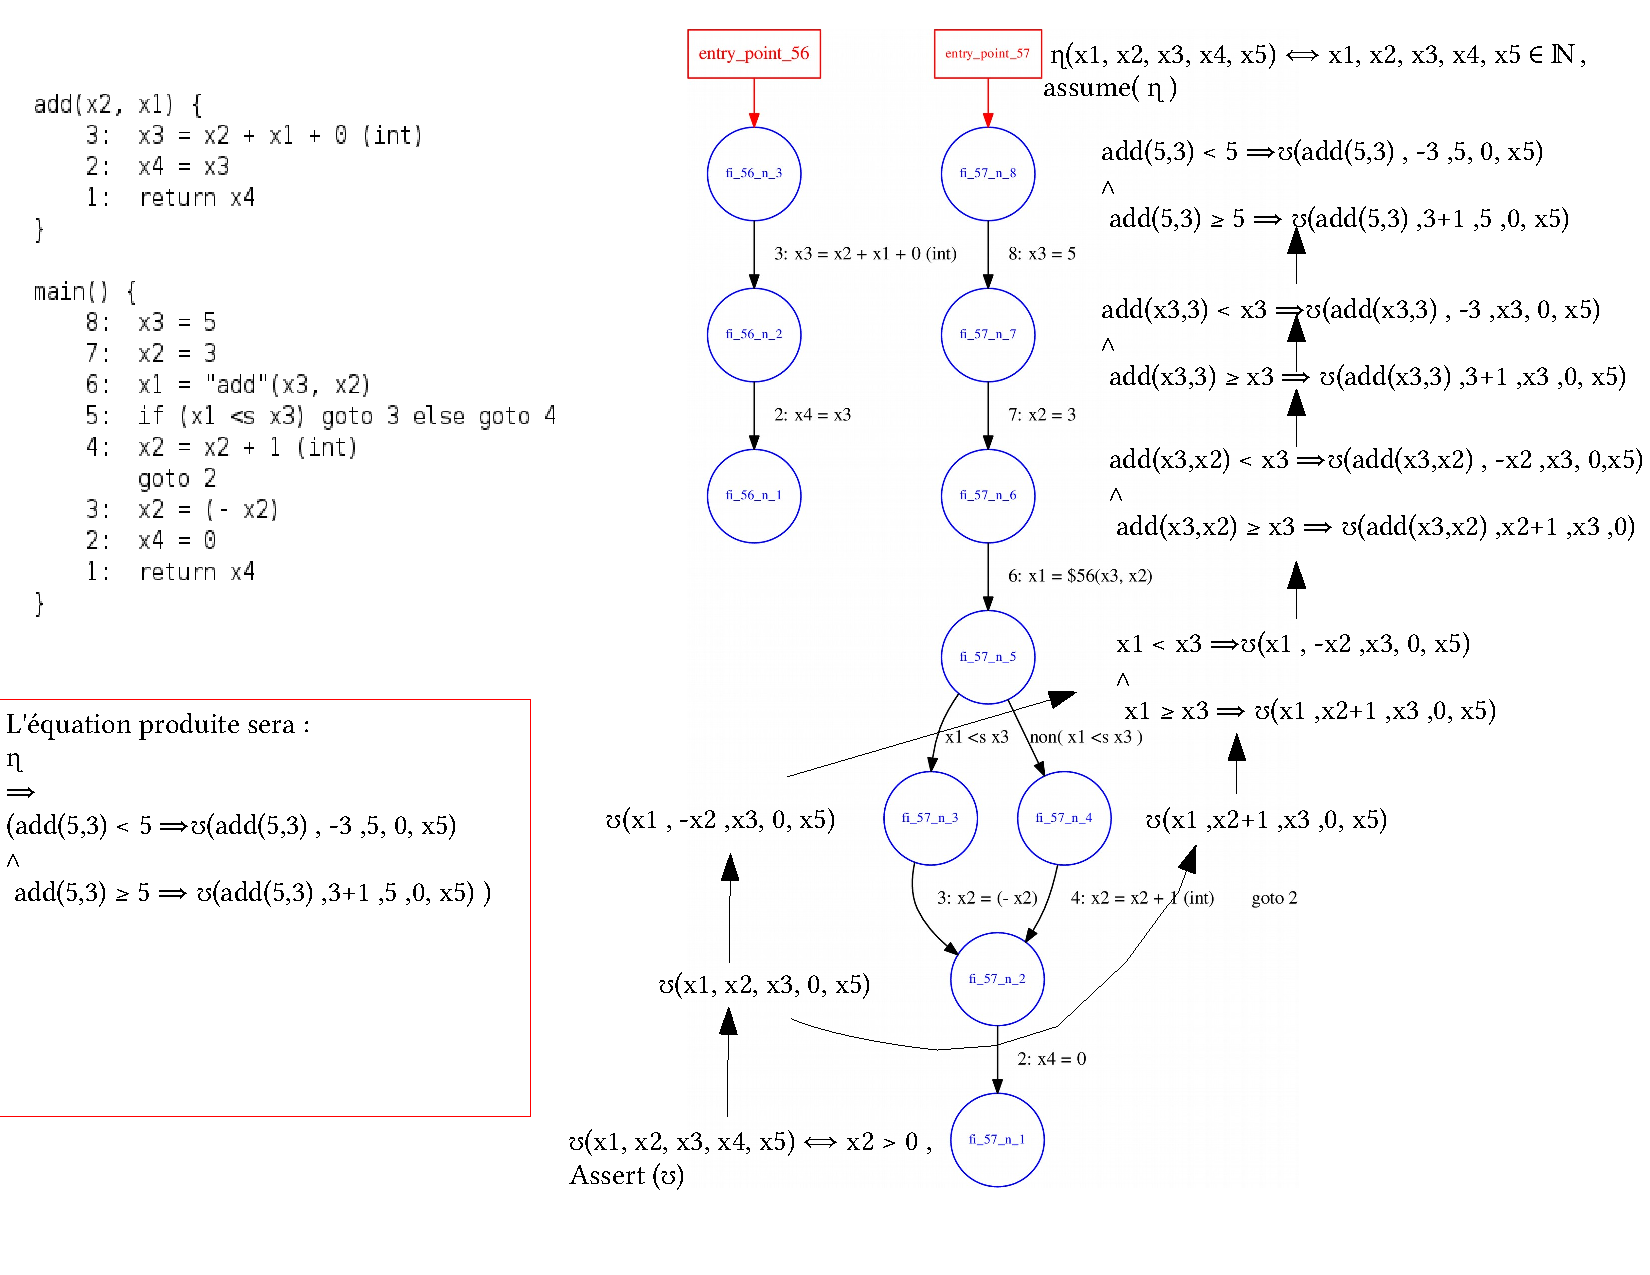
\includegraphics[width=1.2\textwidth]{file_pdf/presentation_no_assert4.pdf} 
%}
\caption{\label{fig:1} Graphe de Flot de Contrôle (CFG) avec le code c associé à côté et les équations logiques qui en découle, noter que toute la formule n'est pas noter a chaque étape.}

\end{figure}


\label{sec:2}
\subsection{D'un graphe de Flot de Contrôle à des formules logiques}


Prenons un exemple plus simple dont le code C et sa traduction RTL sont définis dans la Figure \ref{fig:2} .

\begin{figure}
 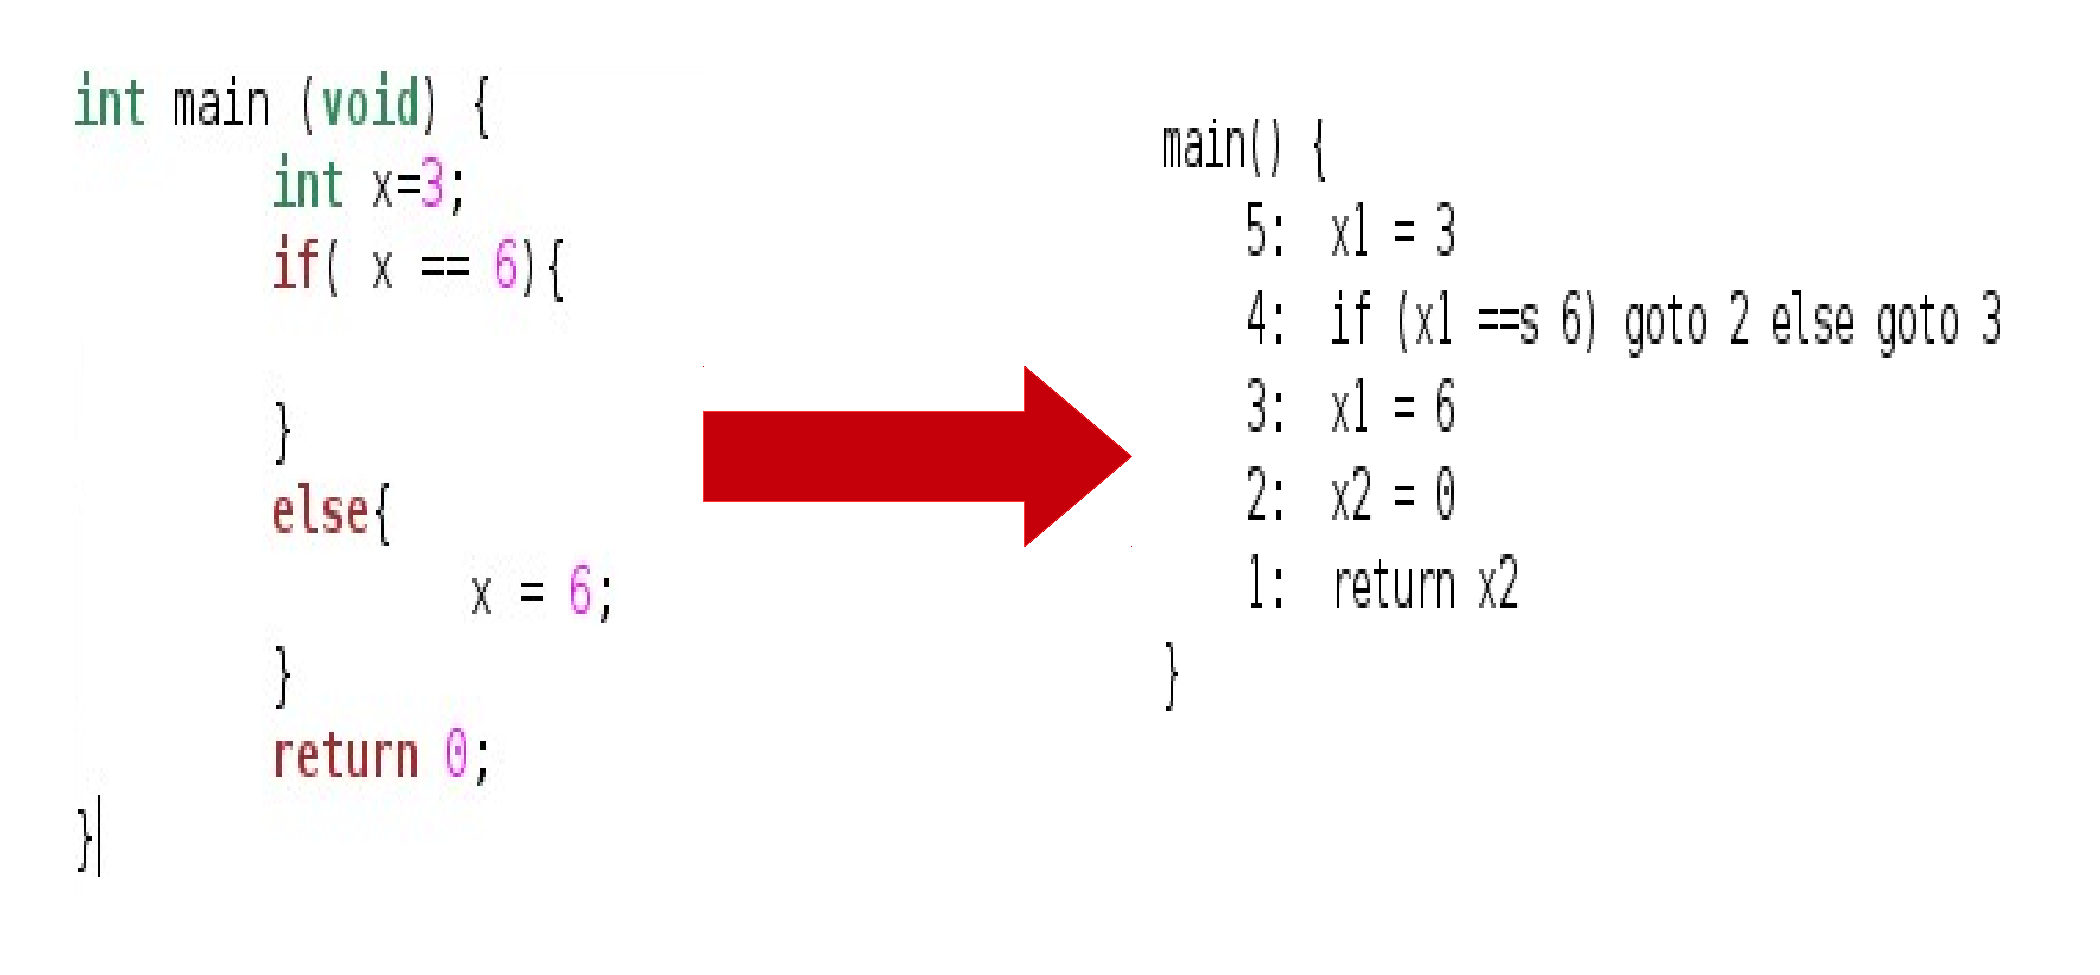
\includegraphics[width=14cm\textwidth, height=5cm\textheight]{file_pdf/presentation_simple_c_to_rtl.pdf}
\caption{ \label{fig:2} transformation du C au RTL}

\end{figure}


Nous allons premièrement rappeler les formules de la logique de Hoare:

Un triplet de Hoare est :
\[  \{\rho\} programme \{\gamma\} \]

où \rho \: représente \: la \: précondition,\: et \: \gamma \: la \: post-condition \: du _: programme.
\smallbreak
Il existe 2 méthodes pour générer les formules logiques d'un programme: \smallbreak
- Strongest Postcondition, qui génère les formules en partant du début du programme vers la fin. \smallbreak
- Weakest Precondition, celle que nous utiliserons qui part de la fin du programme est qui remonte le programme.\smallbreak
%question
Nous allons maintenant expliciter les règles concernants la Weakest Precondition:

Un programme voulant être vérifié doit satisfaire :
\[\forall x, \rho \: \Longrightarrow \:WP(programme,\gamma) \]
Une autre manière de l'écrire est la suivante:
\[WP  : \frac{\rho  \Longrightarrow WP(instr,\gamma)}{ \{\rho\} \: instr \: \{\gamma \} }   \smallbreak
\gamma \: est \: la \: précondition et \rho \: la \: postcondition. \]
%WP (weakest precond) : génération à partir de la fin (assert).

\smallbreak

La séquence :

\[ WP(S1;S2,\gamma) \:  = \: WP(S1,WP(S2,\gamma)\]
\smallbreak

L'affectation:

\[ WP( x \: := \: e, \gamma) \: = \: \gamma[x \leftarrow e]\]
\smallbreak

La condition

\[ WP(\: if \: C \: then \: S1 \: else \: S2, \: \gamma) \: = \: (C \Longrightarrow WP(S1,\gamma)) \: \wedge \: (\lnot C \Longrightarrow WP(S2,\gamma)) \]

\samllbreak
Nous devons maintenant appliquer ces formules à notre graphe issu de la représentation RTL Figure \ref{fig:3}.

\begin{figure}
 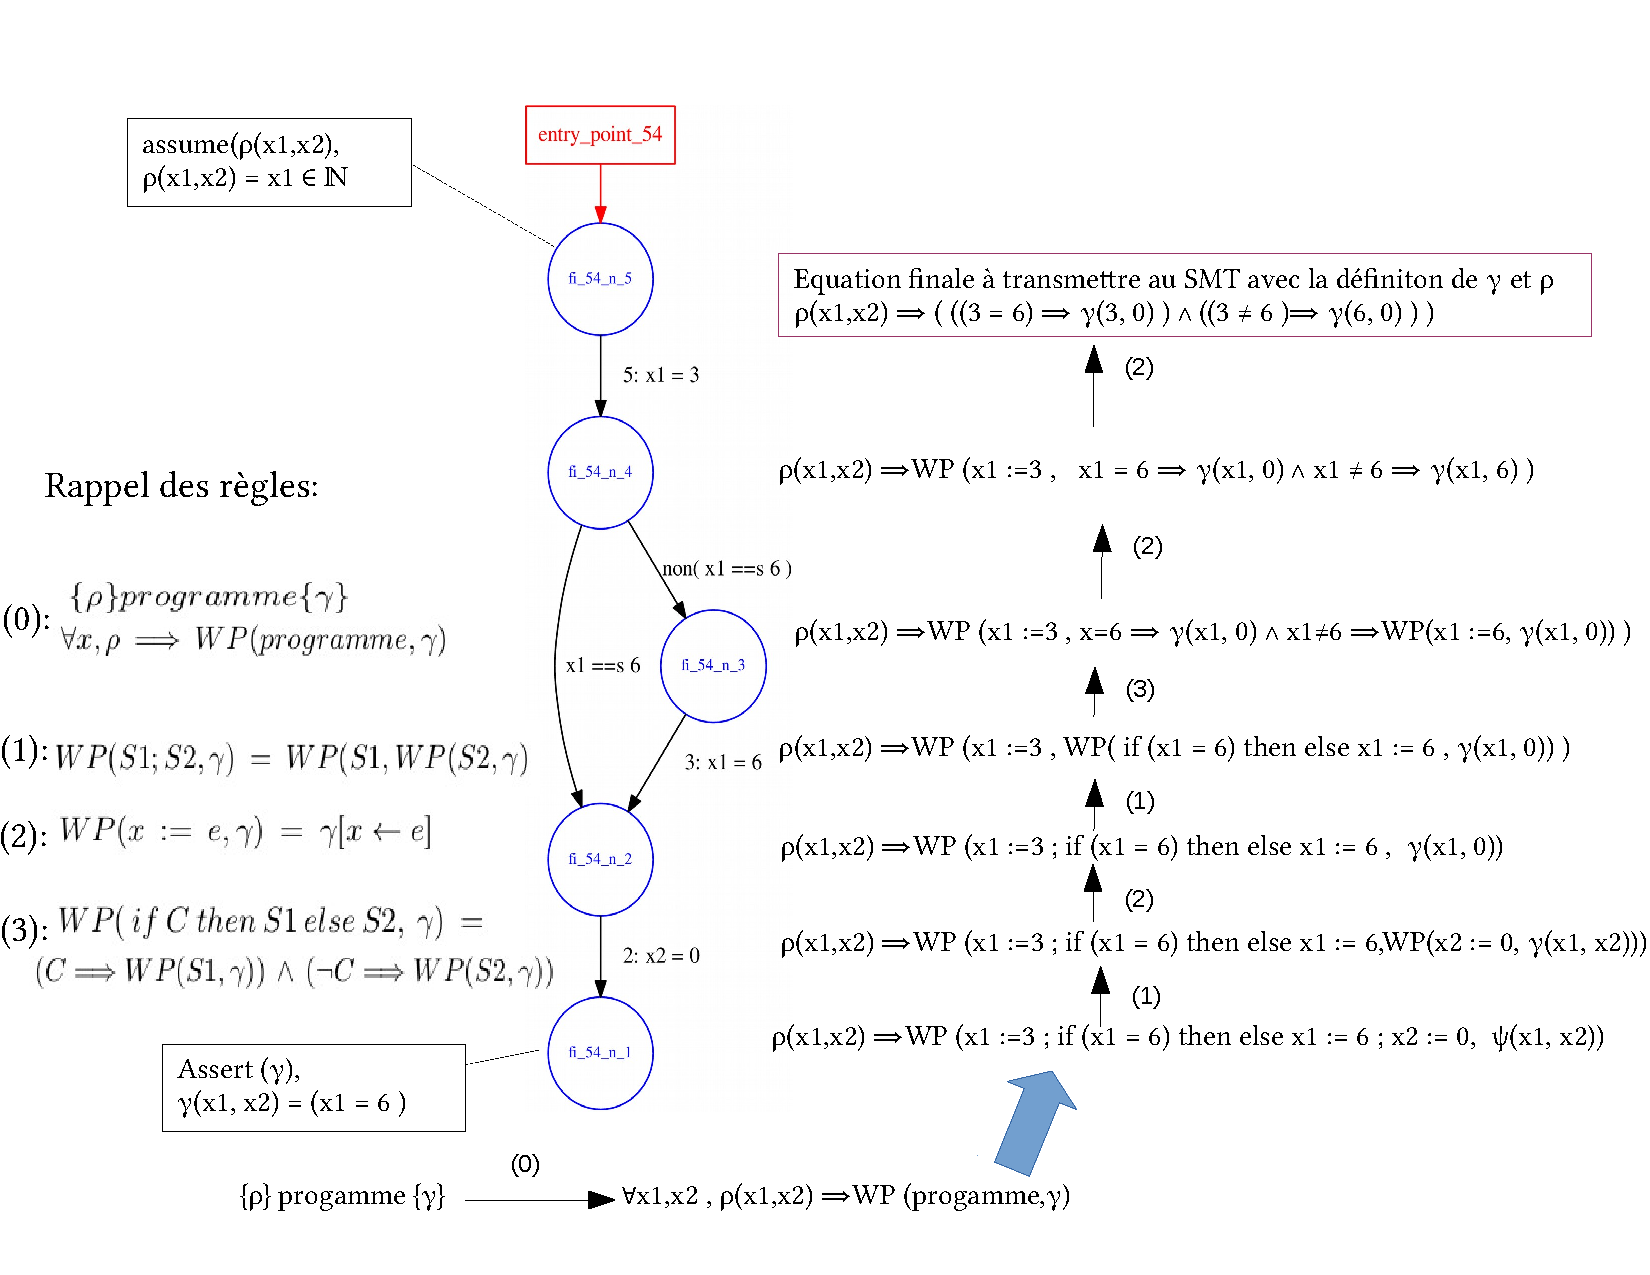
\includegraphics[ height=10cm\textheight]{file_pdf/explication_WP3.pdf}
\caption{\label{fig:3} Construction avec les règles de WP}
%question

\end{figure}



\section{Contribution}
\subsection{principe théorique}

	Nous nous sommes intégrés dans CompCert au premier endroit où il créé un CFG, de manière à utiliser les principes évoqués précedemment, bien que la Logique de Hoare soit déjà définie, pour l'appliquer sur CompCert il faudra réécrire les règles  pour les adapter aux instructions du language intermédiaire que nous exploitons: RTL (Figure \ref{fig:5}).


\subsection{Travail fourni}
\label{sec:2}

	Premièrement il faut d'abord se rattacher à CompCert, un compilateur industriel, comprendre globalement l'architecture du logiciel et comment sont reliés entre eux les différents fichiers afin de finalement travailler dessus. 
	Bien que nous ayons eu facilement un accès aux données nécessaires, cependant cela n'était pas suffisant pour les manipuler librement. En effet modifier quelque chose pour le tester revenait à recompiler CompCert, raison pour laquelle nous avons utilisé une librairie caml particulière (ppx\_deriving.show) pour récupérer la structure de données traité par CompCert.
%ans un premier temps il était necessaire de le récupérer pour travailler dessus 
%Pour les récupérer nous avons du utiliser une librairie ocaml (ppx\_deriving.show) particulière %pour récupérer le code de CompCert. 
	Le principe de la librairie est de générer automatiquement des fonctions capables d'afficher un type, qu'il soit un type somme, enregistrement ou autre. 
Pour cela nous avions besoin de modifier les fichiers où étaient définis ces types que nous voulions afficher, ainsi que les fichiers où l'on definissait les types de bases (Figure 
\ref{fig:4}).

\begin{figure}[b]

 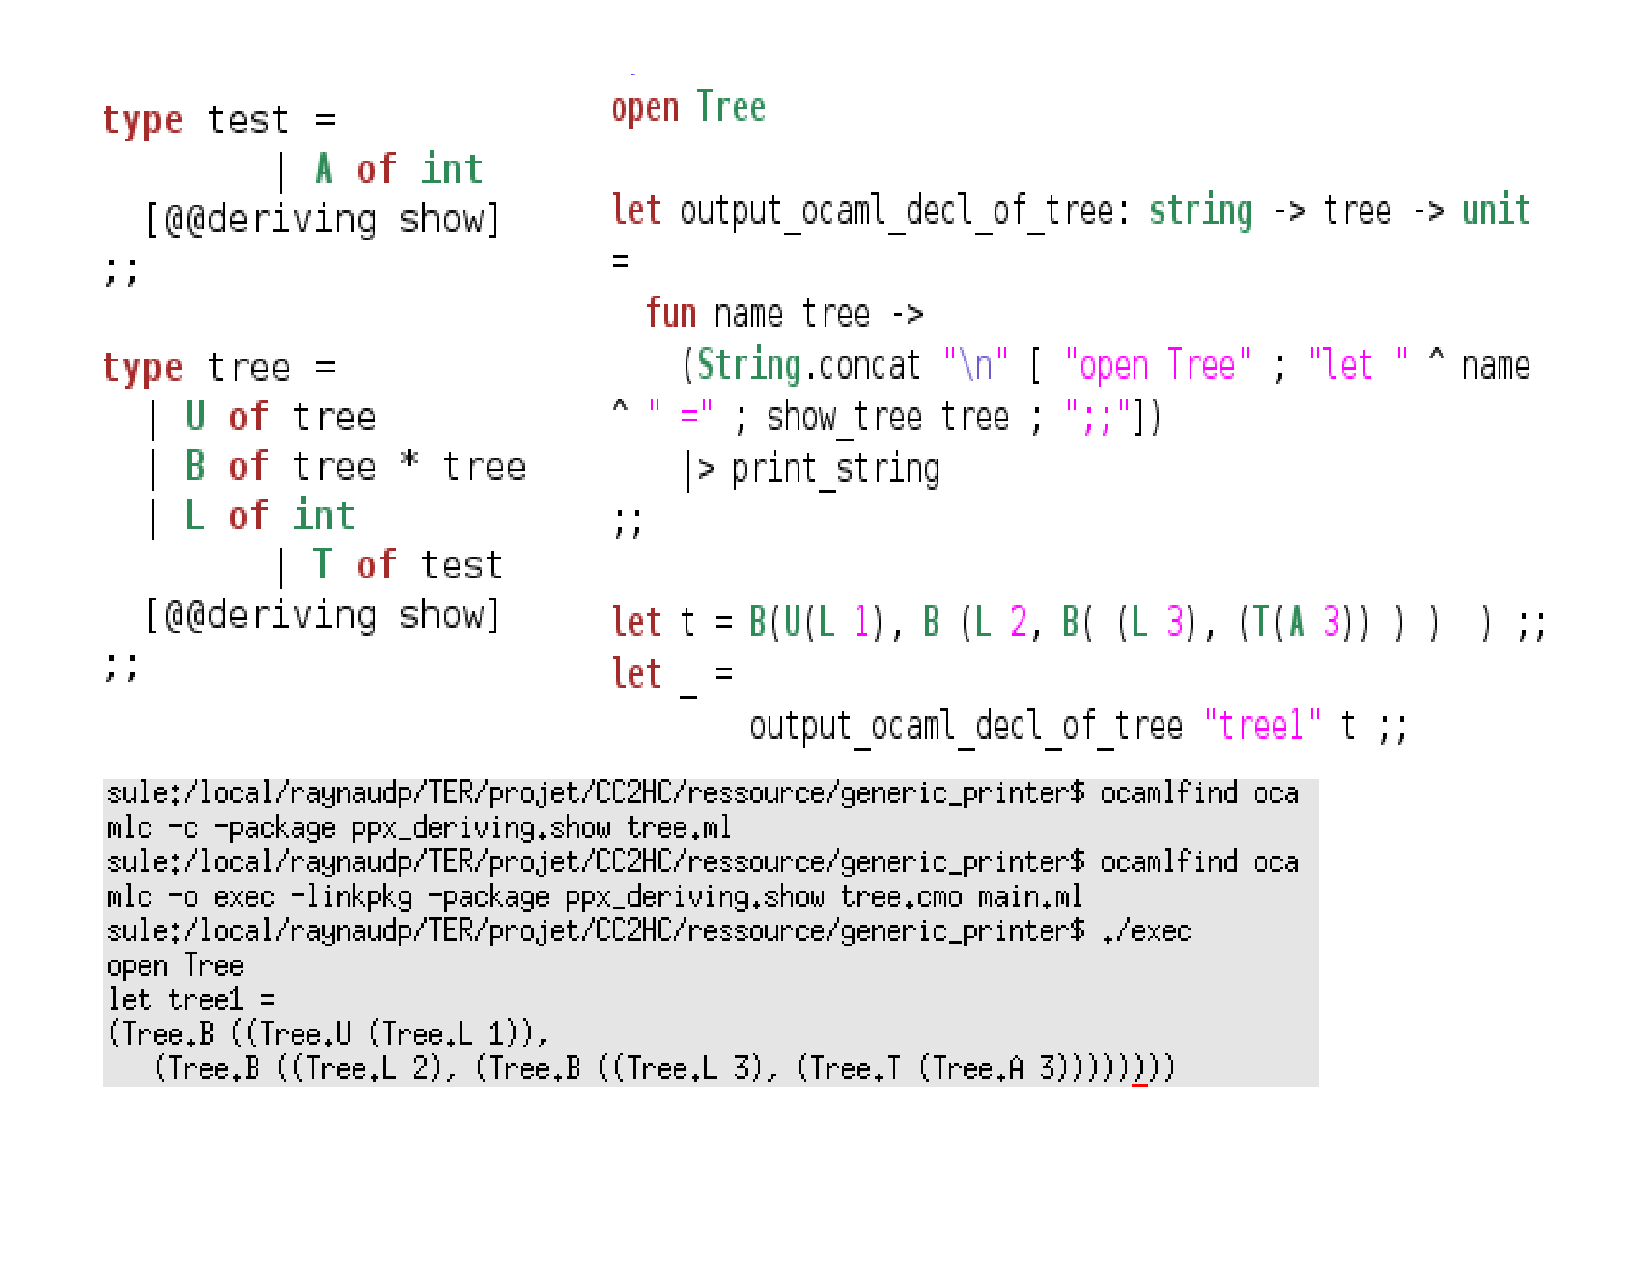
\includegraphics[width=1.1\textwidth]{ressource_generic_printer.pdf}
\caption{\label{fig:4} Exemple d'utilisation de ppx\_deriving.show }

\end{figure}
\smallbreak
%modif
La compilation fût un peu compliquée (annexe \ref{Annexe:1}) mais une fois la structure du code compilé par CompCert extraite, nous obtenons une liste de graphes de flot de contrôle, où chacun d'eux représente une fonction/procédure. (Figure \ref{fig:5})		

\begin{figure}

 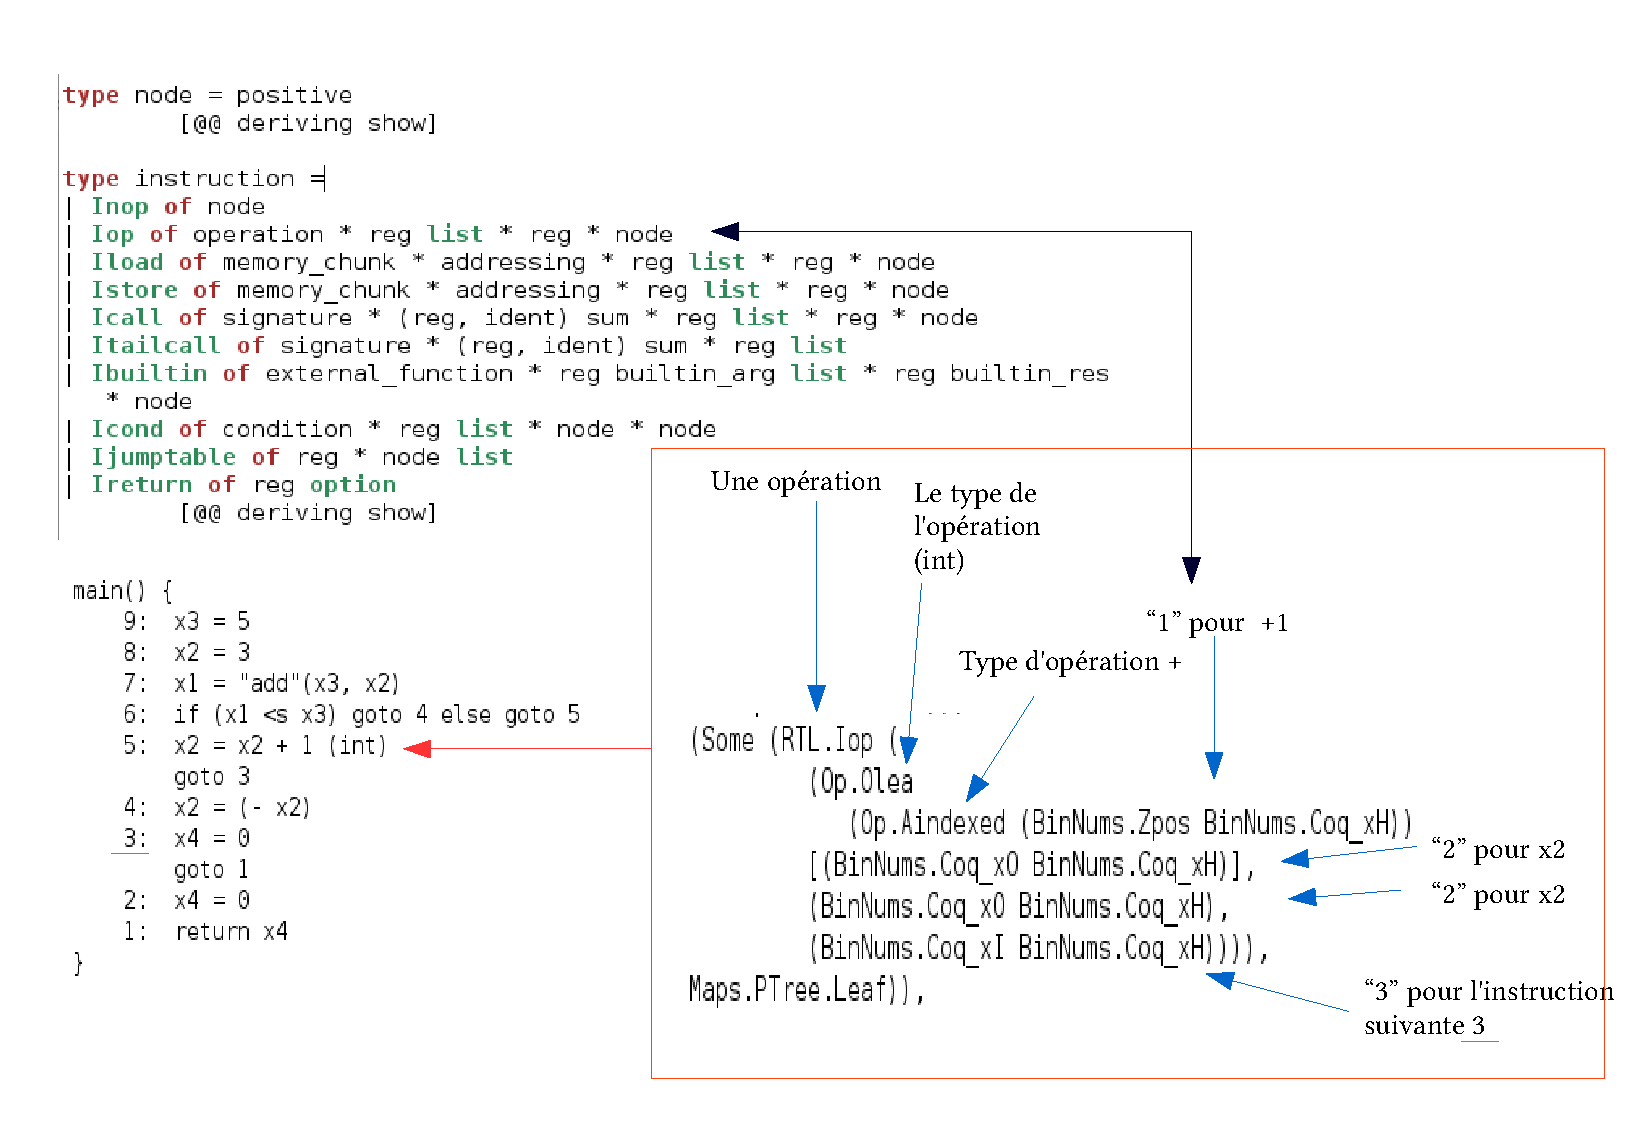
\includegraphics[width=15cm\textwidth,height=13cm \texteheight]{file_pdf/description_instruction2.pdf}
\caption{\label{fig:5} Description d'une opération }

\end{figure}

En retriant les instructions de l'arbre, et en les modifiant nous avons réalisé une première nouvelle structure qui sied mieux à la représentation d'un CFG, une structure par triplet (Figure \ref{fig:6}).
  
\begin{figure}

 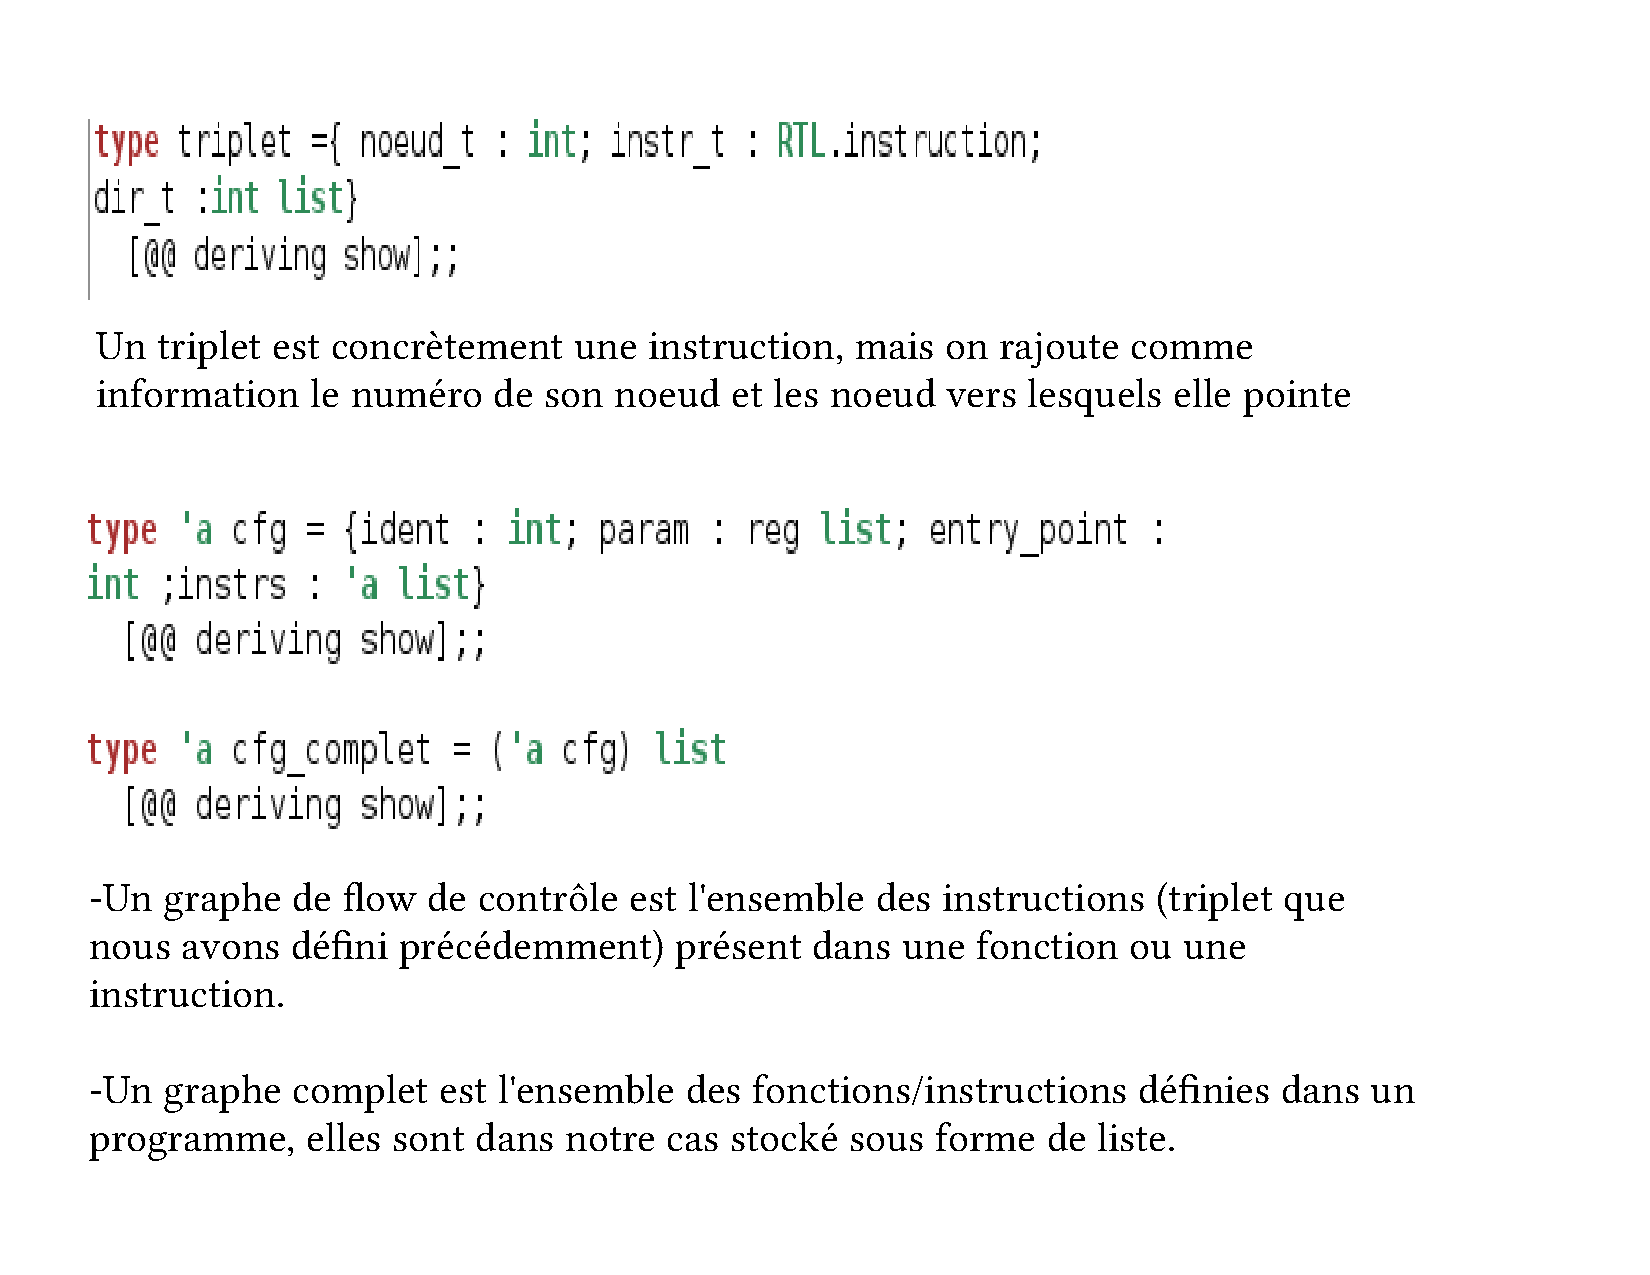
\includegraphics[width=13cm\textwidth,height=8cm \texteheight]{file_pdf/definition_triplet_cfg.pdf}
\caption{\label{fig:6} définition des triplets et cfg }

\end{figure}

Une fois notre arbre de départ transformé en un CFG sous forme de triplet nous avons développé un printer au format .dot permettant d'afficher un graphe grâce au logiciel graphviz (graphe sur les Figures \ref{fig:1} et \ref{fig:3}).
% permettant de créer un fichier .dot et d'afficher sous forme de graphe visuel notre structure de CFG en utilisant le logiciel graphviz. (graphe sur les figure 1 et 3)

%modif question
%En développant un peu plus nous avons réalisé une seconde structure plus en accord avec la logique de Hoare qui se veut de "remonter" le CFG en partant du bas  : une structure de quadruplet .

%EXPLICATION DE LA SECONDE STRUCTURE : ajout des predecesseur 
%
%\underline{est-il necessaire de developper le cfg a quadruplet?}

Maintenant que nous pouvons démarrer sur des bases plus solides, nous devrions developper la génération de clauses de Horn au format du SMT-solver que nous choisirons.




\section{Extensions possibles et probables}
\label{sec:1}
\subsection{\`{A} court terme}
	Le but de ce stage est de commencer ce compilateur du C vers des clauses de Horn en  développant un premier outil capable de générer des clauses pour un sous-ensemble (plutôt simple) d'instructions de C. Mais ce n'est pas une finalité en soit.

\label{sec:2}
\subsection{Sur le moyen terme}
	Une seconde étape serait de compléter cet outil pour être capable de traiter tout le C, comme ce que réalise déjà les autres "verifieur" (SeaHorn, Boogie ...), car si on ne supporte pas toutes les instructions supportés par CompCert, l'outil sera inutilisable (ou peu utilisable). 

\label{sec:3}
\subsection{Pour être synchronisé avec CompCert}
	Une fois que toutes les instruction du C acceptées par CompCert sont traitées au complet il faudra rester dans la même logique que CompCert et prouver ce que nous avons réalisé jusque là. D'après Mr. Périn ce serait le travail d'une thèse. 

	Si le projet arrivait à son terme, alors un programme compilé par CompCert ( et notre outil) serait capable d'avoir des propriétés, et d'être sûr de les maintenir sans craindre de miscompilations.

\section{Annexe}

\subsection{Une compilation compliqué}
\label{Annexe:1}
Cependant les fichiers caml (.ml) contenants les types (les structures) de base de la structure d'un programme et leurs interfaces (.mli), sont générés lors de la compilation (de CompCert), ce qui pose 2 problèmes :\break
- l'effacement de nos fichiers à chaque recompilation de CompCert\break
- la simple modification des .ml ne suffit pas, car l'interface n'est plus en accord avec le fichier caml. La création d'un nouvelle interface pour chaque fichier modifié est donc necessaire.

Nous avons donc décidé de sauvegarder nos fichiers modifiés (.ml) dans un répertoire particulier, les compiler de manière indépendante pour générer leurs interfaces et les fichiers intermédiaires ( .mli, cmi ). Car de la même manière que les .mli, le .cmi dépend des .mli et si nous utilisons les .mli  générés par CompCert au même moment que les .ml, il y aura un conflit entre l'interface et le fichier source et il sera impossile de créer le .cmi qui est necessaire à la compilation. 
Une fois cela réalisé, nous les avons réinjecté au moment opportun dans la compilation de CompCert, pour qu'il créé lui même les .cmo et que l'on soit capable d'afficher la structure que nous voulons, en modifiant légèrement un printer déjà existant.(Figure\ref{fig:7} )

\begin{figure}[t]

 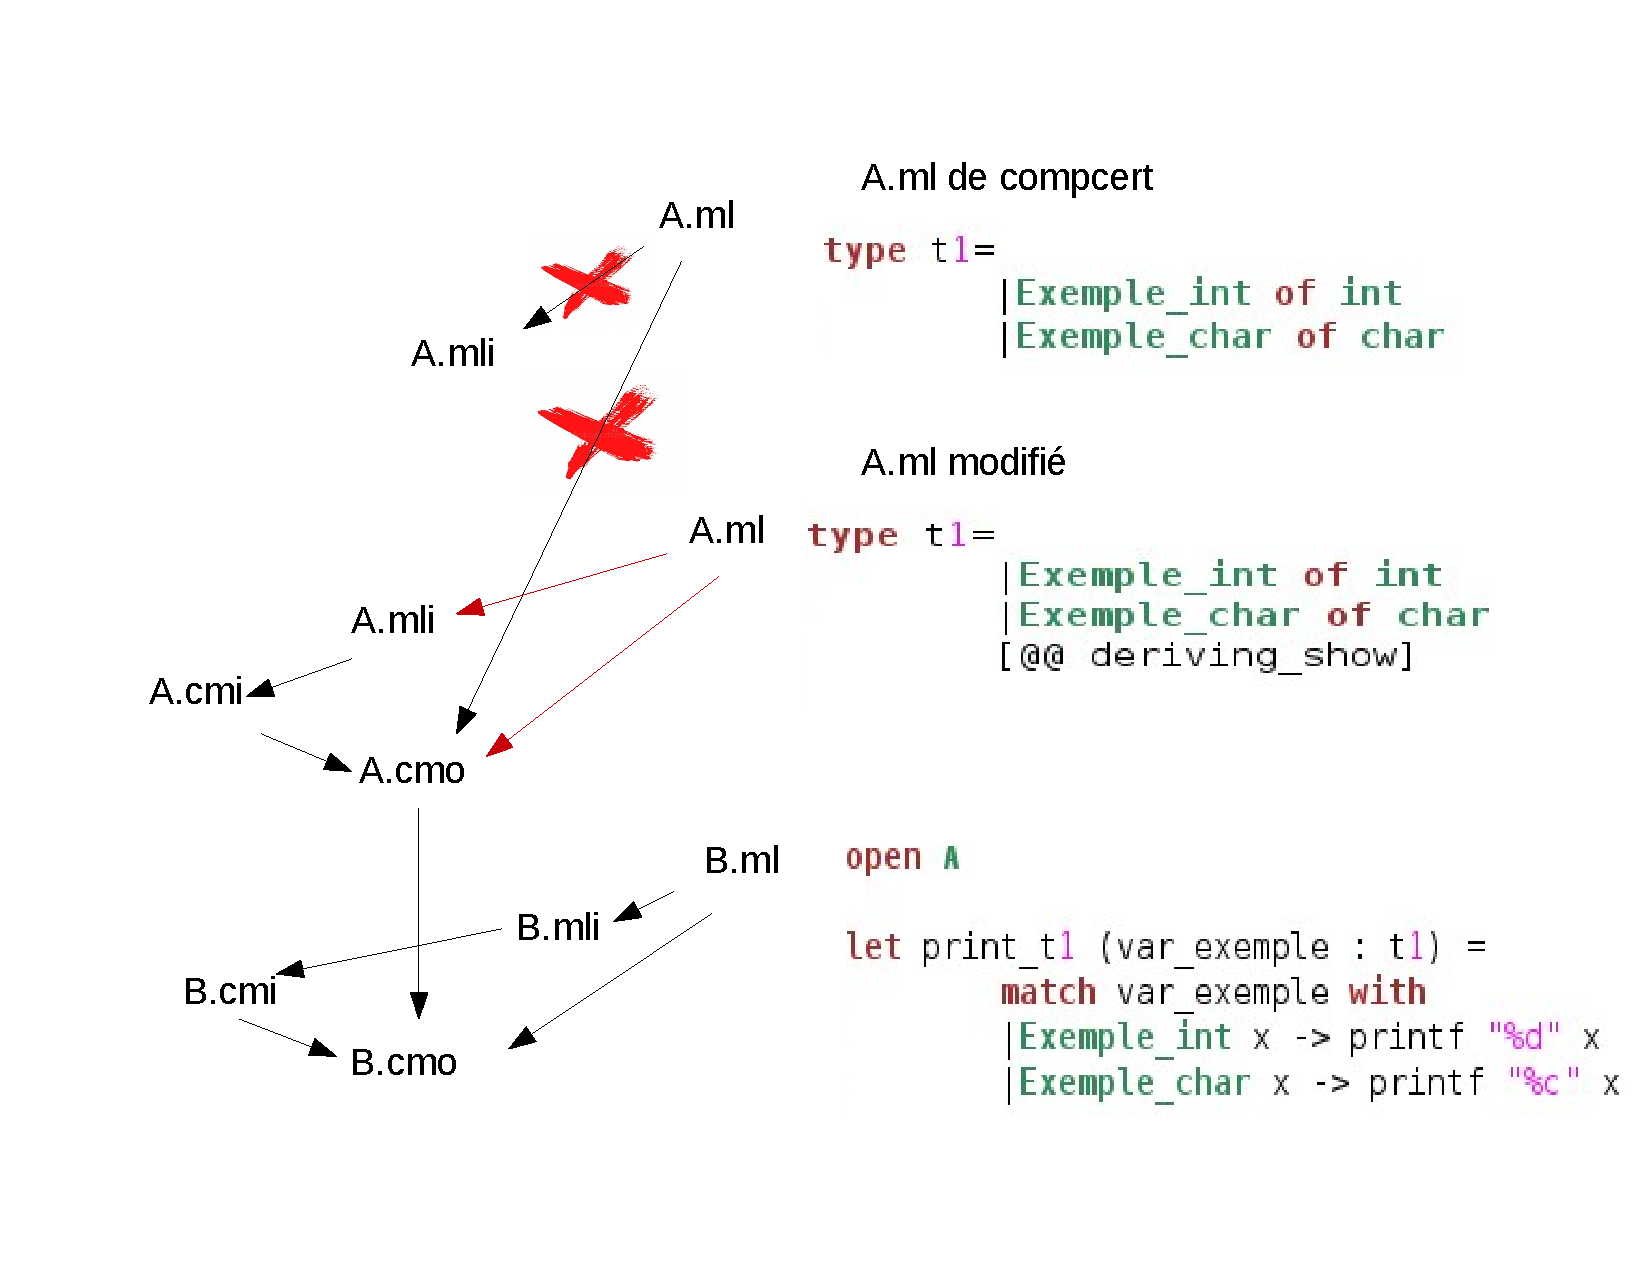
\includegraphics[width=12cm\textwidth,height=8cm \texteheight]{explication_de_la_compilation.pdf}
\caption{\label{fig:7} Exemple simple de la compilation }

\end{figure}

%\label{sec:2}
%\subsection{règles de Hoare}
%Un triplet de Hoare est :
%\[  \{\rho\} instr \{\gamma\} \]
%
%où \rho \: représente \: la \: précondition,\: et \: \gamma \: la \: post \: condition
%
%WP (weakest precond) : génération à partir de la fin (assert).
%
%\[WP  : \frac{\rho  \Longrightarrow WP(instr) (\gamma)}{ \{\rho\} \: instr \: \{\gamma \} }                  \]

%SP (strongest postcondition) : génération a partir du début (assume).

%\[SP  : \frac{ SP(\rho)(instr) \Longrightarrow  (\gamma)}{ \{\rho\} \: instr \: \{\gamma \} }                  \]


%\[Weakening  : \frac{ \rho \Longrightarrow \rho' \:\:  \{\rho'\} \: instr \: \{\gamma'\} \:\: \gamma' \Longrightarrow \gamma}
%{ \{\rho\} \: instr \: \{\gamma \} }                  \]

%\label{sec:3}
%\subsection{règles de WP}

%\[WP [Cond]( \gamma )  \: : \: Cond \: \longrightarrow \: \gamma  } \]  

%j'écrirai les autres règles demain.




%\section{commande latex}
%\label{sec:1}
%\subsection{original}
%Text with citations \cite{RefB} and \cite{RefJ}.

%as required. Don't forget to give each section
%and subsection a unique label (see Sect.~\ref{sec:1}).
%\paragraph{Paragraph headings} Use paragraph headings as needed.
%\begin{equation}
%a^2+b^2=c^2
%\end{equation}

% For one-column wide figures use
%\begin{figure}
% Use the relevant command to insert your figure file.
% For example, with the graphicx package use
% figure caption is below the figure

%\label{fig:1}       % Give a unique label
%\end{figure}
%
% For two-column wide figures use
%\begin{figure*}
% Use the relevant command to insert your figure file.
% For example, with the graphicx package use
% figure caption is below the figure

%\label{fig:2}       % Give a unique label
%\end{figure*}
%
% For tables use
%\begin{table}
% table caption is above the table
%\caption{Please write your table caption here}
%\label{tab:1}       % Give a unique label
% For LaTeX tables use
%\begin{tabular}{lll}
%\hline\noalign{\smallskip}
%first & second & third  \\
%\noalign{\smallskip}\hline\noalign{\smallskip}
%number & number & number \\
%number & number & number \\
%\noalign{\smallskip}\hline
%\end{tabular}
%\end{table}


%\begin{acknowledgements}
%If you'd like to thank anyone, place your comments here
%and remove the percent signs.
%\end{acknowledgements}

% BibTeX users please use one of
%\bibliographystyle{spbasic}      % basic style, author-year citations
%\bibliographystyle{spmpsci}      % mathematics and physical sciences
%\bibliographystyle{spphys}       % APS-like style for physics
%\bibliography{}   % name your BibTeX data base

% Non-BibTeX users please use
\begin{thebibliography}{}
%
% and use \bibitem to create references. Consult the Instructions
% for authors for reference list style.
%
[1] Yang & Al ,"Finding and Understanding Bugs in C Compilers", pages 1-11, 2011\break
\bibitem{RefJ} 
[2] C. A. R. HOARE ,"An Axiomatic Basis for Computer Programming", page 1-6, 1969
% Format for Journal Reference
%Author, Article title, Journal, Volume, page numbers (year)
% Format for books
\bibitem{RefB}
%Author, Book title, page numbers. Publisher, place (year)
% etc
\end{thebibliography}

\end{document}
% end of file template.tex

